% Chapter 2: Theory
\section{理论基础}

\subsection{度量空间与支撑点空间}

\subsubsection{度量空间回顾}

度量空间是一个二元组$(M, d)$,其中$M$是数据对象的集合,$d: M \times M \to \mathbb{R}^+_0$是距离函数,满足:
\begin{itemize}
    \item \textbf{正定性}:$d(x, y) \geq 0$,当且仅当$x = y$时$d(x, y) = 0$
    \item \textbf{对称性}:$d(x, y) = d(y, x)$
    \item \textbf{三角不等式}:$d(x, z) \leq d(x, y) + d(y, z)$
\end{itemize}

\subsubsection{支撑点空间定义}

给定度量空间$(M, d)$和$k$个支撑点$P = \{p_1, p_2, ..., p_k\}$,\textbf{支撑点空间映射}定义为:
\begin{equation}
    F_d^P: M \to \mathbb{R}^k: x^P = F_d^P(x) = (d(x, p_1), d(x, p_2), ..., d(x, p_k))
\end{equation}

对于3个pivot,数据被映射到3维空间:$(d_1, d_2, d_3) = (d(x, p_1), d(x, p_2), d(x, p_3))$。

\subsubsection{支撑点空间的性质}

\textbf{性质1(距离下界)}:对于度量空间中的任意两点$x, y$:
\begin{equation}
    d(x, y) \geq \max_{i} |d(x, p_i) - d(y, p_i)| = d_{\infty}(x^P, y^P)
\end{equation}

即度量空间距离是支撑点空间切比雪夫距离的上界。

\textbf{性质2(范围查询映射)}:度量空间中以$q$为中心、半径$r$的范围查询,映射到支撑点空间后:
\begin{itemize}
    \item 包含于以$q^P$为中心、半径$r$的切比雪夫球中
    \item 即一个边长$2r$的超立方体$\{x^P: \max_i |x_i^P - q_i^P| \leq r\}$
\end{itemize}

\subsection{MVP树原理}

\subsubsection{基本思想}

MVP树(Multiple Vantage Point Tree)由Bozkaya和Ozsoyoglu于1999年提出,是VP树的自然扩展:
\begin{itemize}
    \item \textbf{VP树}:1个pivot,划分为2个部分,记为MVP(1,2)
    \item \textbf{MVP树}:$k$个pivot,每个pivot划分为$f$个部分,记为MVP(k,f)
\end{itemize}

对于MVP(3,2)树(本次实现):
\begin{itemize}
    \item 使用3个pivot:$p_1, p_2, p_3$
    \item 每个pivot将数据划分为2个部分(内球/外球)
    \item 总共产生$2^3 = 8$个子区域
\end{itemize}

\subsubsection{数据划分方式}

MVP树采用\textbf{嵌套球形划分}:
\begin{enumerate}
    \item 按第1个支撑点距离的中位数划分为2个子集
    \item 对每个子集,按第2个支撑点距离的中位数再划分
    \item 对每个子集,按第3个支撑点距离的中位数再划分
    \item 共得到8个子集
\end{enumerate}

子树索引使用二进制编码,如表\ref{tab:mvp-partition}所示。

\begin{table}[htbp]
    \centering
    \caption{MVP树子区域编码}
    \label{tab:mvp-partition}
    \begin{tabular}{ccccc}
        \toprule
        \textbf{Index} & \textbf{Binary} & \textbf{$p_1$ Region} & \textbf{$p_2$ Region} & \textbf{$p_3$ Region} \\
        \midrule
        0 & 000 & Inner & Inner & Inner \\
        1 & 001 & Outer & Inner & Inner \\
        2 & 010 & Inner & Outer & Inner \\
        3 & 011 & Outer & Outer & Inner \\
        4 & 100 & Inner & Inner & Outer \\
        5 & 101 & Outer & Inner & Outer \\
        6 & 110 & Inner & Outer & Outer \\
        7 & 111 & Outer & Outer & Outer \\
        \bottomrule
    \end{tabular}
\end{table}

\subsubsection{剪枝规则}

对于查询$(q, r)$和子树$i$,设:
\begin{itemize}
    \item $d_j = d(q, p_j)$:查询对象到第$j$个pivot的距离
    \item $[L_{i,j}, U_{i,j}]$:子树$i$中数据到第$j$个pivot的距离范围
\end{itemize}

\textbf{排除规则}(任一成立即可排除):
\begin{equation}
    \exists j: d_j + r < L_{i,j} \quad \text{或} \quad d_j - r > U_{i,j}
\end{equation}

\textbf{包含规则}(任一成立则全包含):
\begin{equation}
    \exists j: d_j + U_{i,j} \leq r
\end{equation}

图\ref{fig:mvp-partition}展示了MVP树的嵌套球形划分示意。

\begin{figure}[htbp]
    \centering
    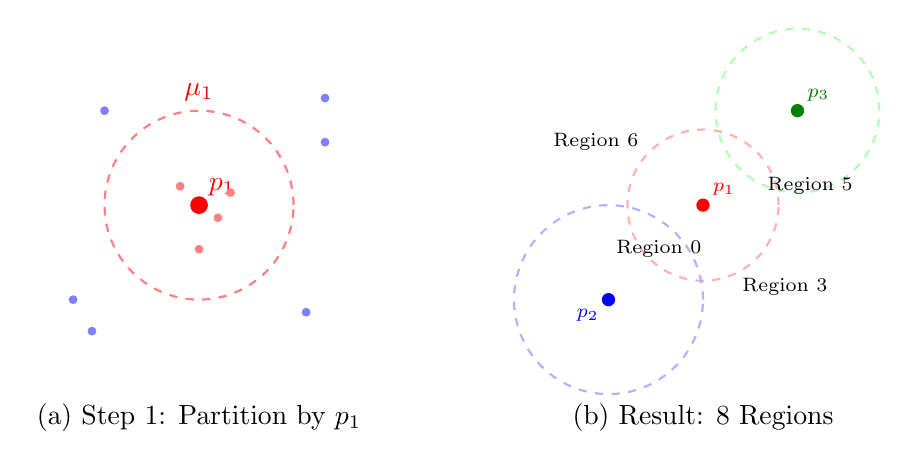
\begin{tikzpicture}[scale=0.8]
        % First pivot division
        \begin{scope}[xshift=0cm]
            \fill[red] (2.5,2.5) circle (4pt) node[above right] {$p_1$};
            \draw[thick,dashed,red!50] (2.5,2.5) circle (1.5);
            \node[red] at (2.5,4.3) {$\mu_1$};
            
            % Data points
            \foreach \x/\y in {2.2/2.8, 2.8/2.3, 2.5/1.8, 3/2.7} {
                \fill[red!50] (\x,\y) circle (2pt);
            }
            \foreach \x/\y in {0.5/1, 4.5/3.5, 1/4, 4.2/0.8, 0.8/0.5, 4.5/4.2} {
                \fill[blue!50] (\x,\y) circle (2pt);
            }
            
            \node[below] at (2.5,-0.5) {(a) Step 1: Partition by $p_1$};
        \end{scope}
        
        % After all three partitions
        \begin{scope}[xshift=8cm]
            \fill[red] (2.5,2.5) circle (3pt) node[above right] {\scriptsize $p_1$};
            \fill[blue] (1,1) circle (3pt) node[below left] {\scriptsize $p_2$};
            \fill[green!50!black] (4,4) circle (3pt) node[above right] {\scriptsize $p_3$};
            
            % Concentric circles (conceptual)
            \draw[thick,dashed,red!30] (2.5,2.5) circle (1.2);
            \draw[thick,dashed,blue!30] (1,1) circle (1.5);
            \draw[thick,dashed,green!30] (4,4) circle (1.3);
            
            % Data regions (simplified)
            \node at (1.8,1.8) {\scriptsize Region 0};
            \node at (3.8,1.2) {\scriptsize Region 3};
            \node at (0.8,3.5) {\scriptsize Region 6};
            \node at (4.2,2.8) {\scriptsize Region 5};
            
            \node[below] at (2.5,-0.5) {(b) Result: 8 Regions};
        \end{scope}
    \end{tikzpicture}
    \caption{MVP树嵌套球形划分示意}
    \label{fig:mvp-partition}
\end{figure}

\subsection{完全广义超平面树原理}

\subsubsection{基本思想}

完全广义超平面树(Complete GHT, CGHT)由毛睿教授于2014年提出,核心思想是:

\begin{quote}
    \textbf{充分利用pivot对之间的距离差信息进行划分}
\end{quote}

对于2个pivot $p_1, p_2$,原始GH树只利用了$d(x, p_1) - d(x, p_2)$的\textbf{符号}(正/负),而CGHT还利用其\textbf{大小}。

对于3个pivot,定义:
\begin{align}
    \delta_{12} &= d(x, p_1) - d(x, p_2) \\
    \delta_{13} &= d(x, p_1) - d(x, p_3) \\
    \delta_{23} &= d(x, p_2) - d(x, p_3) = \delta_{13} - \delta_{12}
\end{align}

只需要2个独立变量$(\delta_{12}, \delta_{13})$即可表示所有距离差信息。

\subsubsection{4路划分策略}

基于$\delta_{12}$和$\delta_{13}$的符号进行4路划分,如表\ref{tab:cgh-partition}所示。

\begin{table}[htbp]
    \centering
    \caption{CGH树4路划分}
    \label{tab:cgh-partition}
    \begin{tabular}{cccl}
        \toprule
        \textbf{Index} & \textbf{$\delta_{12}$} & \textbf{$\delta_{13}$} & \textbf{Geometric Meaning} \\
        \midrule
        0 & $< 0$ & $< 0$ & Farthest from $p_1$ \\
        1 & $\geq 0$ & $< 0$ & Farthest from $p_3$ \\
        2 & $< 0$ & $\geq 0$ & Farthest from $p_2$ \\
        3 & $\geq 0$ & $\geq 0$ & Closest to $p_1$ \\
        \bottomrule
    \end{tabular}
\end{table}

\subsubsection{剪枝规则}

基于GH树剪枝规则的扩展。对于查询$(q, r)$,设:
\begin{align}
    \delta_{12}^q &= d(q, p_1) - d(q, p_2) \\
    \delta_{13}^q &= d(q, p_1) - d(q, p_3)
\end{align}

对于子树$i$,其$\delta_{12}$范围为$[L_{12}^i, U_{12}^i]$,$\delta_{13}$范围为$[L_{13}^i, U_{13}^i]$。

\textbf{排除条件}(任一成立即可排除):
\begin{equation}
    \delta_{12}^q - 2r > U_{12}^i \quad \text{或} \quad \delta_{12}^q + 2r < L_{12}^i
\end{equation}
\begin{equation}
    \delta_{13}^q - 2r > U_{13}^i \quad \text{或} \quad \delta_{13}^q + 2r < L_{13}^i
\end{equation}

图\ref{fig:cgh-partition}展示了CGH树的超平面划分示意。

\begin{figure}[htbp]
    \centering
    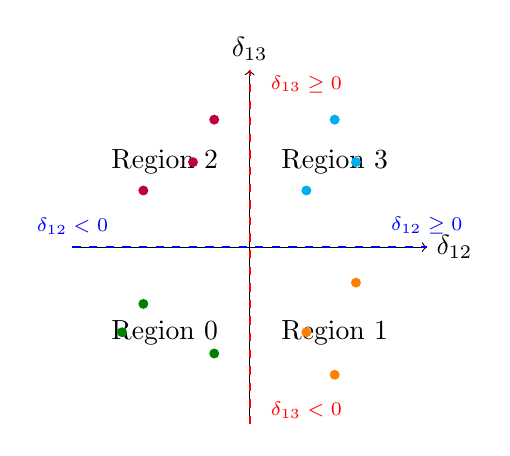
\begin{tikzpicture}[scale=0.9]
        % Coordinate system in delta space
        \draw[->] (-2.5,0) -- (2.5,0) node[right] {$\delta_{12}$};
        \draw[->] (0,-2.5) -- (0,2.5) node[above] {$\delta_{13}$};
        
        % Partition lines
        \draw[thick,dashed,blue] (-2.5,0) -- (2.5,0);
        \draw[thick,dashed,red] (0,-2.5) -- (0,2.5);
        
        % Regions
        \node at (-1.2,-1.2) {Region 0};
        \node at (1.2,-1.2) {Region 1};
        \node at (-1.2,1.2) {Region 2};
        \node at (1.2,1.2) {Region 3};
        
        % Annotations
        \node[blue] at (-2.5,0.3) {\scriptsize $\delta_{12} < 0$};
        \node[blue] at (2.5,0.3) {\scriptsize $\delta_{12} \geq 0$};
        \node[red] at (0.8,-2.3) {\scriptsize $\delta_{13} < 0$};
        \node[red] at (0.8,2.3) {\scriptsize $\delta_{13} \geq 0$};
        
        % Data points example
        \foreach \x/\y in {-1.5/-0.8, -0.5/-1.5, -1.8/-1.2} {
            \fill[green!50!black] (\x,\y) circle (2pt);
        }
        \foreach \x/\y in {0.8/-1.2, 1.5/-0.5, 1.2/-1.8} {
            \fill[orange] (\x,\y) circle (2pt);
        }
        \foreach \x/\y in {-0.8/1.2, -1.5/0.8, -0.5/1.8} {
            \fill[purple] (\x,\y) circle (2pt);
        }
        \foreach \x/\y in {0.8/0.8, 1.5/1.2, 1.2/1.8} {
            \fill[cyan] (\x,\y) circle (2pt);
        }
    \end{tikzpicture}
    \caption{CGH树在$(\delta_{12}, \delta_{13})$空间中的4路划分}
    \label{fig:cgh-partition}
\end{figure}

\subsection{完全线性划分原理}

\subsubsection{基本思想}

完全线性划分的核心思想是:

\begin{quote}
    既然数据已经映射到支撑点空间(多维实数空间),就可以使用传统的多维索引方法进行划分。
\end{quote}

\textbf{线性划分}:使用线性超平面$\sum_i a_i x_i = c$对支撑点空间进行划分。

最简单的线性划分是\textbf{正交划分}:
\begin{itemize}
    \item 按$d_1$的中位数划分
    \item 按$d_2$的中位数划分
    \item 按$d_3$的中位数划分
    \item 共产生$2^3 = 8$个子区域
\end{itemize}

\subsubsection{数据结构}

线性划分树内部节点存储:
\begin{itemize}
    \item 3个支撑点
    \item 3个维度的划分阈值(中位数)
    \item 8棵子树
    \item 每个子树在各维度的距离范围$[L_i^j, U_i^j]$
\end{itemize}

\subsubsection{剪枝规则}

查询对象在支撑点空间中的坐标为$q^P = (d_1^q, d_2^q, d_3^q)$。

查询区域是以$q^P$为中心的边长$2r$的立方体(切比雪夫球):
\begin{equation}
    \{(x_1, x_2, x_3): |x_i - d_i^q| \leq r, i=1,2,3\}
\end{equation}

\textbf{排除规则}:若存在任意维度$j$使得:
\begin{equation}
    d_j^q + r < L_i^j \quad \text{或} \quad d_j^q - r > U_i^j
\end{equation}
则子树$i$可以排除。

图\ref{fig:lp-partition}展示了线性划分树在支撑点空间中的划分。

\begin{figure}[htbp]
    \centering
    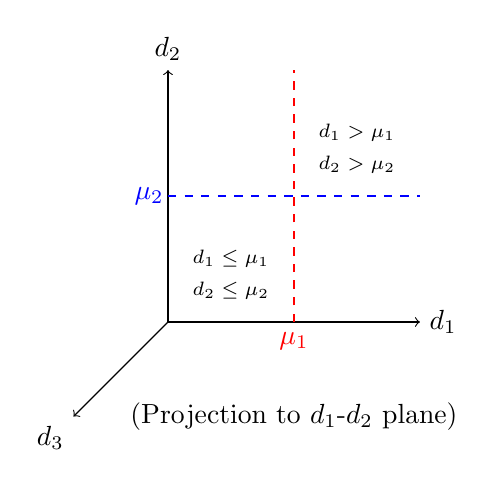
\begin{tikzpicture}[scale=0.8]
        % 3D coordinate system (isometric view)
        \draw[->] (0,0) -- (4,0) node[right] {$d_1$};
        \draw[->] (0,0) -- (0,4) node[above] {$d_2$};
        \draw[->] (0,0) -- (-1.5,-1.5) node[below left] {$d_3$};
        
        % Partition planes (simplified 2D projection)
        \draw[dashed,red] (2,0) -- (2,4);
        \draw[dashed,blue] (0,2) -- (4,2);
        
        % Threshold labels
        \node[red] at (2,-0.3) {$\mu_1$};
        \node[blue] at (-0.3,2) {$\mu_2$};
        
        % Regions
        \node at (1,1) {\scriptsize $d_1 \leq \mu_1$};
        \node at (1,0.5) {\scriptsize $d_2 \leq \mu_2$};
        \node at (3,3) {\scriptsize $d_1 > \mu_1$};
        \node at (3,2.5) {\scriptsize $d_2 > \mu_2$};
        
        % Note
        \node at (2,-1.5) {(Projection to $d_1$-$d_2$ plane)};
    \end{tikzpicture}
    \caption{线性划分树在支撑点空间中的正交划分($d_1$-$d_2$平面投影)}
    \label{fig:lp-partition}
\end{figure}

\subsection{三种索引的理论对比}

表\ref{tab:theory-compare}从多个维度对比了三种索引的特性。

\begin{table}[htbp]
    \centering
    \caption{三种多Pivot索引的理论对比}
    \label{tab:theory-compare}
    \begin{tabular}{lccc}
        \toprule
        \textbf{Feature} & \textbf{MVP Tree} & \textbf{CGH Tree} & \textbf{LP Tree} \\
        \midrule
        Partition Space & Metric Space & Metric Space & Pivot Space \\
        Partition Boundary & Spheres & Hyperplanes & Linear Hyperplanes \\
        Number of Children & $2^k = 8$ & $2^{k-1} = 4$ & $2^k = 8$ \\
        Distance Info Used & $d(x, p_i)$ & $d(x, p_i) - d(x, p_j)$ & $(d_1, d_2, d_3)$ \\
        Containment Rule & Yes & No & Yes (approx.) \\
        \bottomrule
    \end{tabular}
\end{table}
